\PassOptionsToPackage{unicode=true}{hyperref} % options for packages loaded elsewhere
\PassOptionsToPackage{hyphens}{url}
%
\documentclass[
]{article}
\usepackage{lmodern}
\usepackage{amssymb,amsmath}
\usepackage{ifxetex,ifluatex}
\ifnum 0\ifxetex 1\fi\ifluatex 1\fi=0 % if pdftex
  \usepackage[T1]{fontenc}
  \usepackage[utf8]{inputenc}
  \usepackage{textcomp} % provides euro and other symbols
\else % if luatex or xelatex
  \usepackage{unicode-math}
  \defaultfontfeatures{Scale=MatchLowercase}
  \defaultfontfeatures[\rmfamily]{Ligatures=TeX,Scale=1}
\fi
% use upquote if available, for straight quotes in verbatim environments
\IfFileExists{upquote.sty}{\usepackage{upquote}}{}
\IfFileExists{microtype.sty}{% use microtype if available
  \usepackage[]{microtype}
  \UseMicrotypeSet[protrusion]{basicmath} % disable protrusion for tt fonts
}{}
\makeatletter
\@ifundefined{KOMAClassName}{% if non-KOMA class
  \IfFileExists{parskip.sty}{%
    \usepackage{parskip}
  }{% else
    \setlength{\parindent}{0pt}
    \setlength{\parskip}{6pt plus 2pt minus 1pt}}
}{% if KOMA class
  \KOMAoptions{parskip=half}}
\makeatother
\usepackage{xcolor}
\IfFileExists{xurl.sty}{\usepackage{xurl}}{} % add URL line breaks if available
\IfFileExists{bookmark.sty}{\usepackage{bookmark}}{\usepackage{hyperref}}
\hypersetup{
  pdftitle={What Data Science Can Do For You},
  pdfauthor={The Data Science Team at PSRC},
  pdfborder={0 0 0},
  breaklinks=true}
\urlstyle{same}  % don't use monospace font for urls
\usepackage[margin=1in]{geometry}
\usepackage{graphicx,grffile}
\makeatletter
\def\maxwidth{\ifdim\Gin@nat@width>\linewidth\linewidth\else\Gin@nat@width\fi}
\def\maxheight{\ifdim\Gin@nat@height>\textheight\textheight\else\Gin@nat@height\fi}
\makeatother
% Scale images if necessary, so that they will not overflow the page
% margins by default, and it is still possible to overwrite the defaults
% using explicit options in \includegraphics[width, height, ...]{}
\setkeys{Gin}{width=\maxwidth,height=\maxheight,keepaspectratio}
\setlength{\emergencystretch}{3em}  % prevent overfull lines
\providecommand{\tightlist}{%
  \setlength{\itemsep}{0pt}\setlength{\parskip}{0pt}}
\setcounter{secnumdepth}{-2}
% Redefines (sub)paragraphs to behave more like sections
\ifx\paragraph\undefined\else
  \let\oldparagraph\paragraph
  \renewcommand{\paragraph}[1]{\oldparagraph{#1}\mbox{}}
\fi
\ifx\subparagraph\undefined\else
  \let\oldsubparagraph\subparagraph
  \renewcommand{\subparagraph}[1]{\oldsubparagraph{#1}\mbox{}}
\fi

% set default figure placement to htbp
\makeatletter
\def\fps@figure{htbp}
\makeatother


\title{What Data Science Can Do For You}
\author{The Data Science Team at PSRC}
\date{}

\begin{document}
\maketitle

\begin{figure}
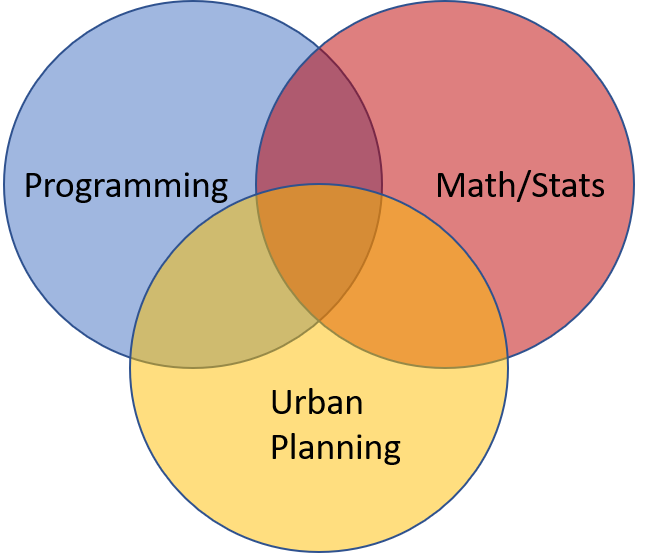
\includegraphics[width=9.25in]{C:/Users/SChildress/Documents/GitHub/data-science/what_we_can_do/DataScience} \caption{PSRC Data Science skills}\label{fig:unnamed-chunk-1}
\end{figure}

\hypertarget{build-apps-to-visualize-and-explain-data}{%
\subsection{Build apps to visualize and explain
data}\label{build-apps-to-visualize-and-explain-data}}

\emph{Examples:}

\href{http://dataexplorer.psrc.org/household-travel-survey}{Household
Travel Survey Data Explorer}

\href{http://aws-linux:3838/covid19-dashboard/}{COVID-19 Dashboard}

\href{http://aws-linux/soundcast_dash}{SoundCast Model Output
Visualization}

\hypertarget{manage-and-organize-your-data}{%
\subsection{Manage and organize your
data}\label{manage-and-organize-your-data}}

Our team has been building a data warehouse with the goal of having
better organized, easy-to-use, and well-documented data. The data
warehouse establishes a standard location and format for our data. We
would love to add your data to the warehouse over time.

\hypertarget{automate-manual-processes}{%
\subsection{Automate manual processes}\label{automate-manual-processes}}

\begin{enumerate}
\def\labelenumi{\arabic{enumi}.}
\item
  Automate complex or repetitive GIS workflows. For example, some data
  may need to be updated quarterly and in this case should be automated.
\item
  Replace complex, hard-to-follow spreadsheets that do critical
  calculations with more documented and easier to replicate processes.
\item
  Capture the expertise and skill of team members by codifying the steps
  they have developed over many years.
\end{enumerate}

\hypertarget{help-in-data-analysis-and-visualization}{%
\subsection{Help in data analysis and
visualization}\label{help-in-data-analysis-and-visualization}}

Some data analysis and visualization may require scripting, and we can
jump in and help.

\hypertarget{find-and-pull-new-andor-common-data-sources-using-code}{%
\subsection{Find and pull new and/or common data sources using
code}\label{find-and-pull-new-andor-common-data-sources-using-code}}

New planning data sources are coming online everyday. We can script
processes to pull from innovative and big data repositories. We can also
schedule these processes to periodically occur to get the latest data
with little overhead.

\emph{Examples:}

\begin{itemize}
\tightlist
\item
  Using google data, we found the distance to the nearest grocery store
  from any location. We used this in displacement risk analysis to show
  which locations were at risk for displacement because they had many
  amenities like grocery stores nearby.
\item
  Census data extractions can be performed in a more automated, less
  laborious way
\item
  Using the google data,we found travel times between pairs of locations
  to analyze household travel survey data
\end{itemize}

\hypertarget{teach-basic-scripting-and-statistical-skills-so-you-can-do-all-these-things-too}{%
\subsection{Teach basic scripting and statistical skills so you can do
all these things
too!}\label{teach-basic-scripting-and-statistical-skills-so-you-can-do-all-these-things-too}}

\hypertarget{who-are-we}{%
\subsection{Who are we?}\label{who-are-we}}

Our data science group team members are Polina Butrina, Suzanne
Childress, Christy Lam, Craig Helmann, Michael Jensen, Diana Martinez,
and Chris Peak. We are all proficient to advanced programmers. Our team
has expertise in programming in R, Python, T-SQL, CSS, and C\#, among
other languages. We have expertise in SQL Server and database management
systems. We also have expertise in GIS, statistics, machine learning,
math, and modeling.

\end{document}
